\subsubsection{Camberline Parametrization}

%% Disable the logo in the lower right corner:
% \hidelogo

\hidelogo
% \begin{frame}{Camberline parametrization}
%     \vspace{-0.5cm}
%     \begin{columns}
%         \column{0.5\textwidth}
%             \begin{block}{Camberline parameters}
%                 \begin{itemize}
%                     \item $\chi_1$: metal inlet angle
%                     \item $\chi_2$: metal outlet angle 
%                     \item $\gamma$: stagger angle
%                 \end{itemize}
%             \end{block}
%             \vspace{-0.4cm}
%             \begin{block}{Camberline formulation}
%                 \tiny{
%                 \begin{itemize}
%                     % \item $a = a_{(\chi_1, \chi_2, \gamma)}$
%                     % \item $b = b_{(\chi_1, \chi_2, \gamma)}$
%                     % \item $n = n_{(\chi_1, \chi_2, \gamma)}$
%                     \item $n = \frac{tan(\chi_2) + tan(\chi_1)}{tan(\gamma)}$
%                     \item $a = \frac{tan(\chi_2)}{n}$
%                     \item $b =  - \frac{tan(\chi_1)}{n}$
%                     \item $y = a \cdot x^n + b \cdot (1 - x)^n$
%                     \item $y^{\prime} = a \cdot n \cdot x^{n-1} - b \cdot n \cdot (1 - x)^{n - 1}$
%                     \item $\boldsymbol{n} = 
%                     \begin{bmatrix}
%                         - \frac{y^{\prime}}{\sqrt{1 + (y^{\prime})^2}} \\
%                         \frac{1}{\sqrt{1 + (y^{\prime})^2}}
%                     \end{bmatrix}$
%                 \end{itemize}
%                 }
%             \end{block}
%         \column{0.5\textwidth}
%             % \begin{block}{Camberline variables}
%                 % \begin{itemize}
%                     % \item $n = \frac{tan(\chi_2) + tan(\chi_1)}{tan(\gamma)}$
%                     % \item $a = \frac{tan(\chi_2)}{n}$
%                     % \item $b =  - \frac{tan(\chi_1)}{n}$
%                 % \end{itemize}
%             % \end{block}
%             \begin{figure}
%                 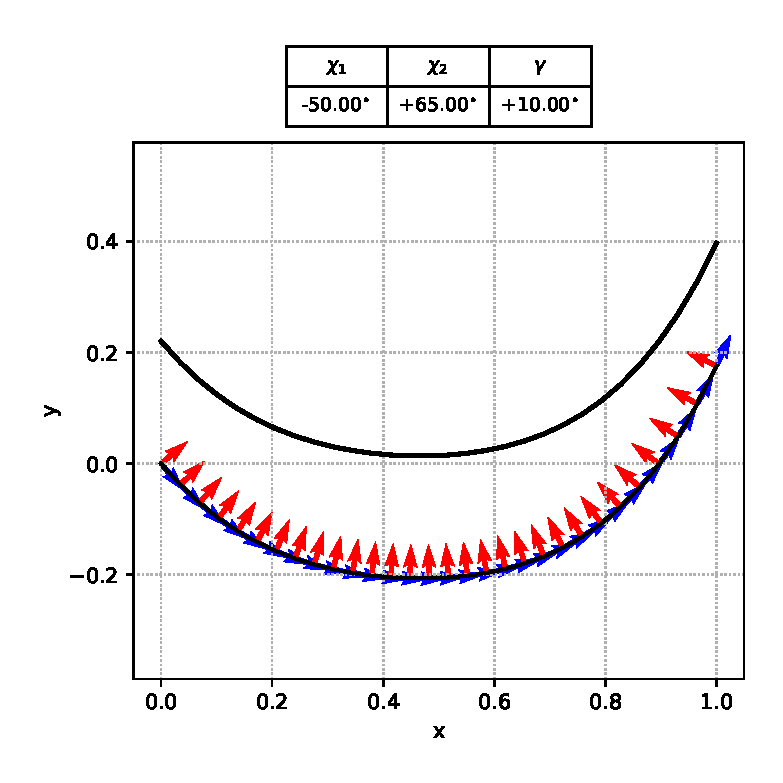
\includegraphics[width=0.8\textwidth]{images/camberline/camberline01.eps}
%             \end{figure}
%     \end{columns}
% \end{frame}   

\begin{frame}{Camberline parametrization}
    \vspace{-0.5cm}
    \begin{columns}
        \column{0.5\textwidth}
            \begin{figure}
                \centering
                \includegraphics[width=\textwidth]{./images/cLine1.eps}
            \end{figure}
        \column{0.5\textwidth}
            \begin{figure}
                \includegraphics[width=\textwidth]{./images/cLine2.eps}
            \end{figure}
    \end{columns}
\end{frame}   

% \subsubsection{Profile Parametrization}
% \begin{frame}{Profile parametrization}
%     \vspace{1cm}
%     \begin{block}{Profile thickness, $\zeta$}
%         Kulfan parametrization studies the thickness distribution using shape functions.
%         \begin{itemize}
%             \setlength\itemsep{0.3cm}
%             \item Class function: $C_{(x)}$
%             \item Shape function: $S_{(x, i, N)}$
%             \item Trailing edge radius thickness distribution: $\zeta_{TE} \cdot x$
%             \item Total shape function: $\zeta_{(x)}$
%         \end{itemize}
%     \end{block}

%     % \begin{block}{Profile properties}
%         % \begin{itemize}
%             % \item Thickness distribution with respect to the Bernstein function: $S_{(x, 0, 2)}$                 
%             % \item The trailing edge radius thickness, $\zeta_{TE_{(x)}}$, is been added normally to the camberline using a linear distribution 
%             % \item The leading edge radius is expressed only by the $A_0$ parameter
%             % \item The wedge angle, $\beta$, is expressed only by the $A_N$ parameter
%         % \end{itemize}
%     % \end{block}
% \end{frame}

\begin{frame}{Bernstein functions and class function}
    % \vspace{-4cm}
    \begin{columns}
        \column{0.5\textwidth}
        \vspace{-0.5cm} 
        \begin{equation*}
            S_{(x, i, N)} = A_i \cdot \frac{N!}{(N - i)! \cdot i!} \cdot x^i \cdot (1 - x)^{N - 1}
        \end{equation*}
        \vspace{-0.5cm}
        \begin{figure}
            % \includegraphics[width=\textwidth]{images/profileLine/bernstein.eps}
            \includegraphics[width=\textwidth]{./images/bernstein.eps}
        \end{figure}
        \column{0.5\textwidth}
        \begin{equation*}
            C_{(x)} = x^{0.5} \cdot (1 - x)^{1.0}
        \end{equation*}
        \begin{figure}
            % \includegraphics[width=\textwidth]{images/profileLine/shapeFunction.eps}
            \includegraphics[width=\textwidth]{./images/class.eps}
        \end{figure}
    \end{columns}
\end{frame}

\begin{frame}{Blades - \Romannum{1}}
    % \vspace{1cm}
    \begin{figure}
        \hspace*{-0.8cm}
        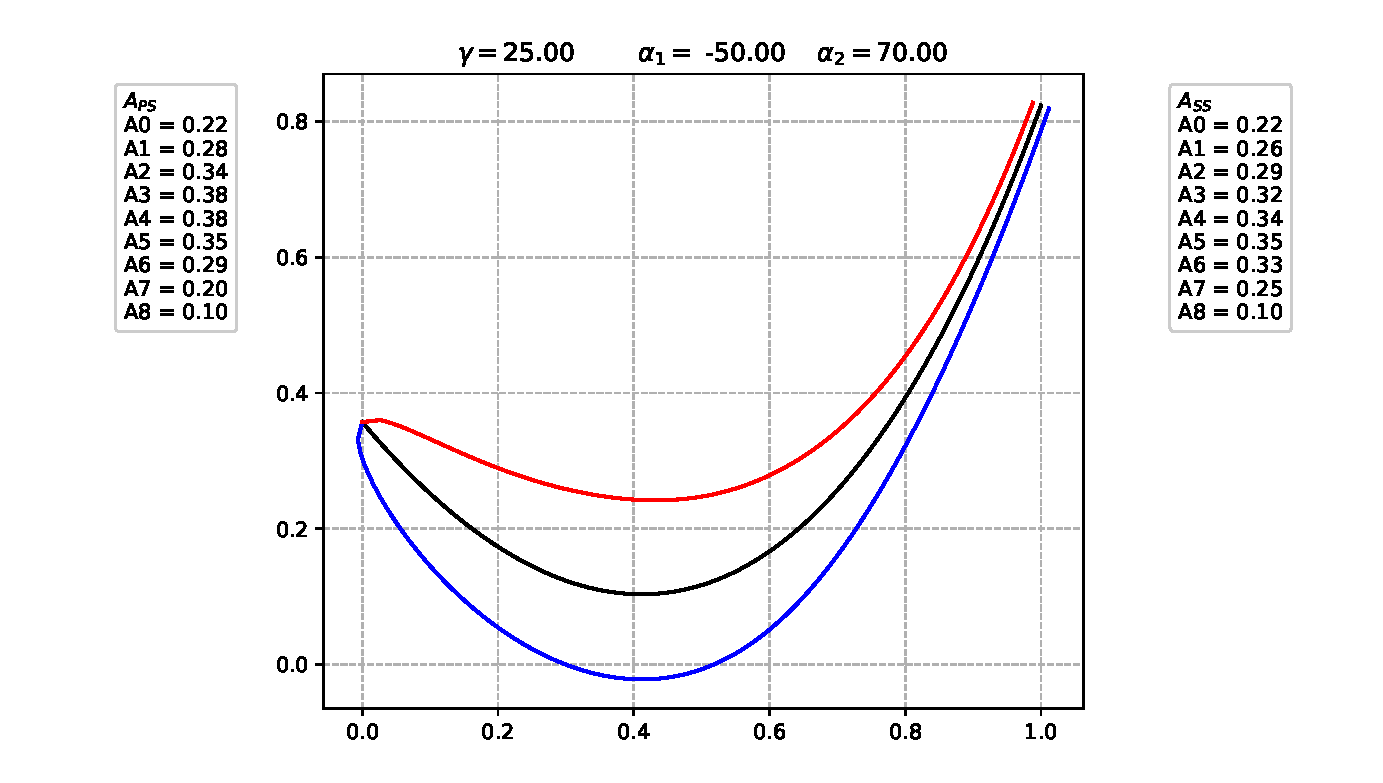
\includegraphics[width=1.2\textwidth, trim=3cm 0cm 0cm 0cm, clip]{./images/blade1.eps}
    \end{figure}
\end{frame}

\begin{frame}{Blades - \Romannum{2}}
    \begin{figure}
        \hspace*{-0.8cm}
        \includegraphics[width=1.2\textwidth, trim=3cm 0cm 0cm 0cm, clip]{./images/blade2.eps}
    \end{figure}
\end{frame}

% \begin{frame}{Kulfan thickness functions}
%     Kulfan thickness distribution is computed using $C_{(x)}$ and $S_{(x, i, N)}$:
%     \begin{equation}
%         \zeta_{(x)} = \sum_{i = 0}^N S_{(x, i, N)} \cdot C_{(x)} \notag
%     \end{equation}
%     \vspace{-2cm}
%     \begin{figure}
%         % 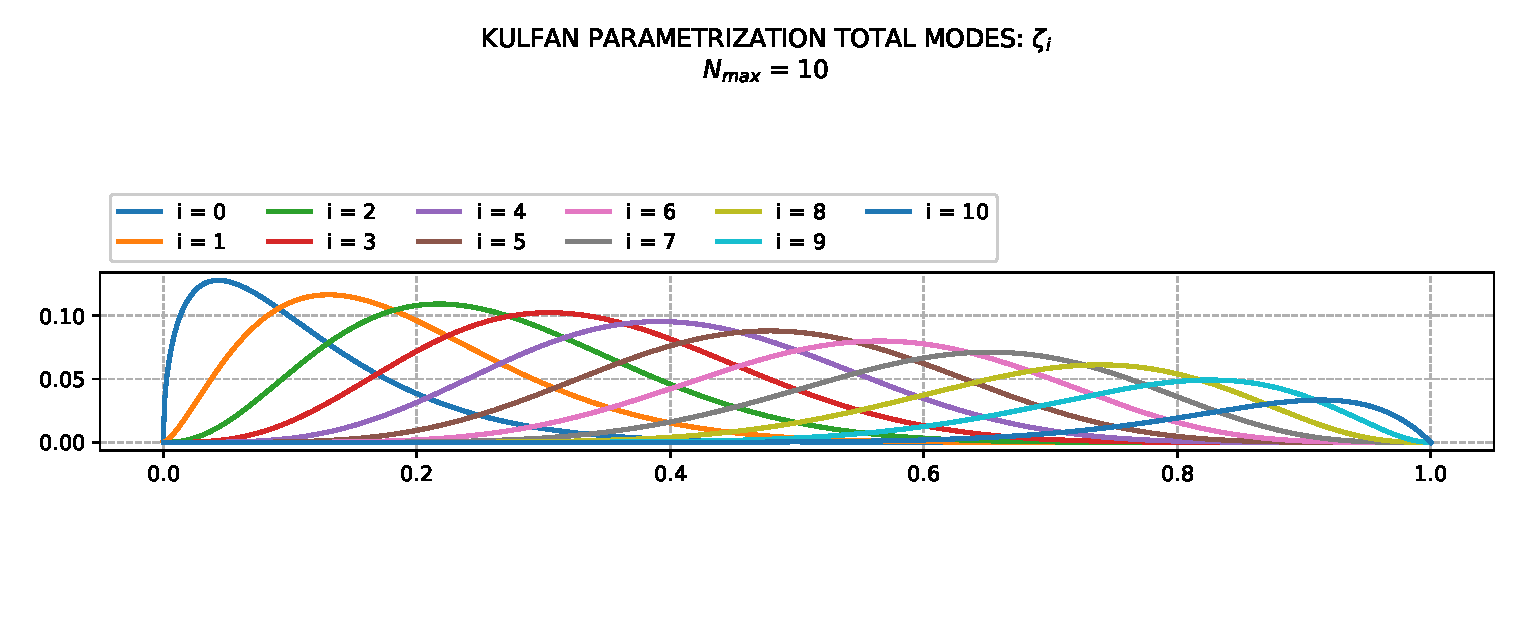
\includegraphics[width=\textwidth]{images/profileLine/kulfan.eps}
%         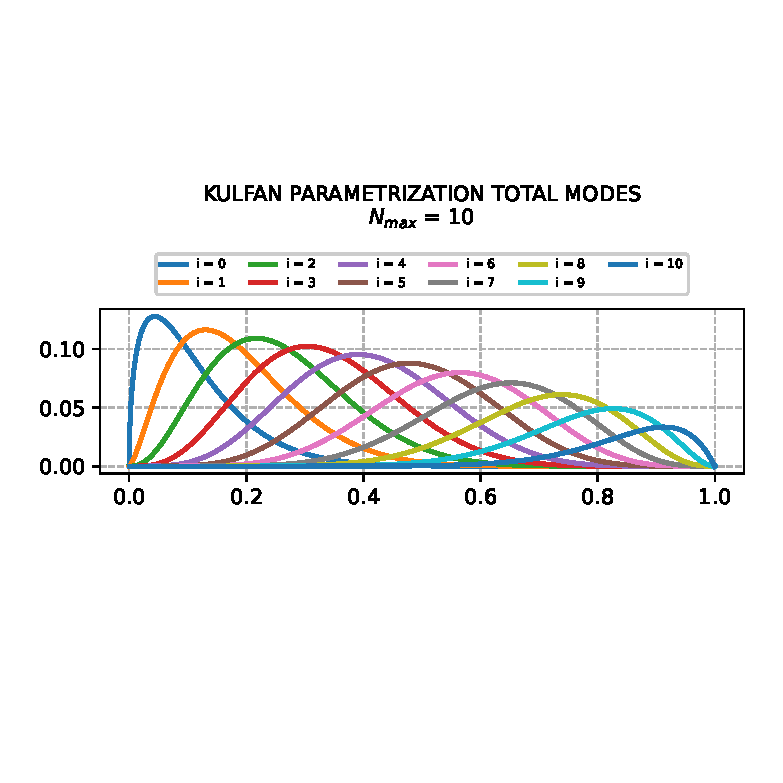
\includegraphics[scale=0.8]{./images/kulfanFunction.eps}
%     \end{figure}
% \end{frame}

% \begin{frame}{Thickness distribution and scaling}
%     \begin{block}{Pressure/suction side generation $(\pm)$}
%         \vspace*{-0.6cm}
%         \begin{align*}
%             \zeta_{TOT_{(x)}} & = \zeta_{(x)} + \zeta_{TE} \cdot x \\
%             x_{PS/SS}         & = x_{camberline} \pm n_x \cdot \zeta_{TOT_{(x)}} \cdot S_{(x, 0, 2)} \\ 
%             y_{PS/SS}         & = y_{camberline} \pm n_y \cdot \zeta_{TOT_{(x)}} \cdot S_{(x, 0, 2)} + \zeta_{(x)} \cdot \big[1 - S_{(x, 0, 2)}\big]
%         \end{align*}
%     \end{block}
%     \vspace{-0.9cm}
%     \begin{columns}
%         \column{0.5\textwidth}
%             \begin{figure}
%                 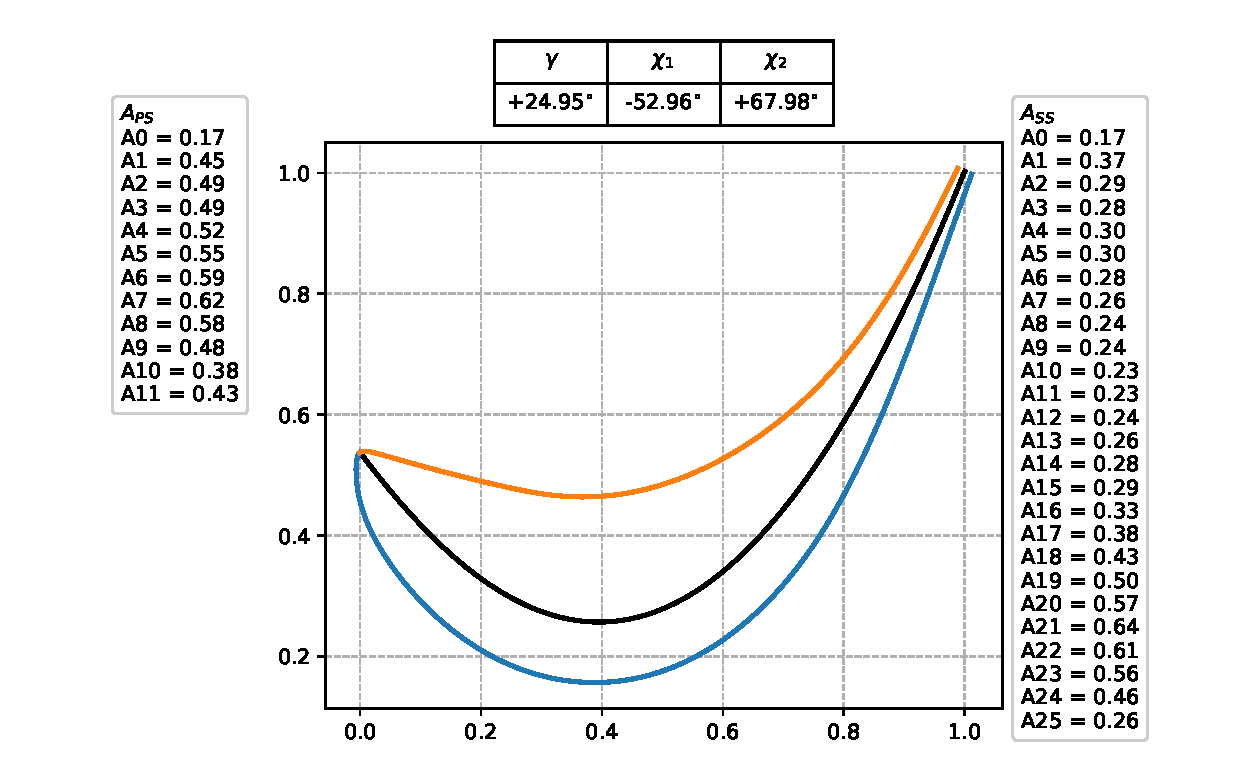
\includegraphics[width=\textwidth]{images/profileLine/blade01.eps}
%             \end{figure}
%         \column{0.5\textwidth}
%             \begin{figure}
%                 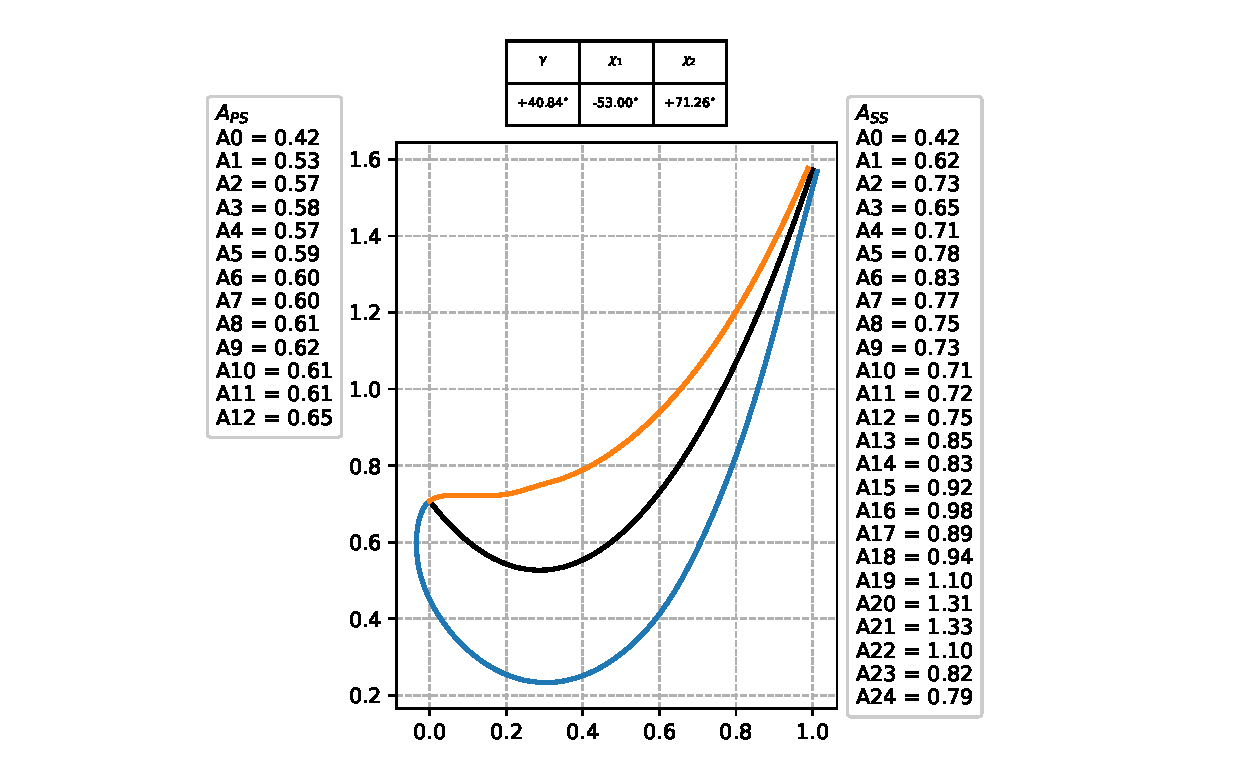
\includegraphics[width=\textwidth]{images/profileLine/blade02.eps}
%             \end{figure}
%     \end{columns}
% \end{frame}